%-------------------------------------------------------------------------------
% 请勿删除本注释
% Free Response Question 1
%
% 指引:
% 如在小问之前有通用问题描述,请放置于此
%-------------------------------------------------------------------------------
\begin{figure}[h]
\centering
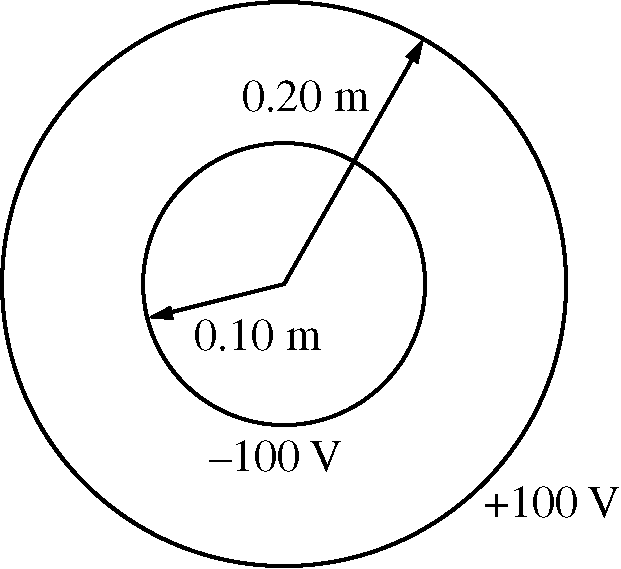
\includegraphics[scale=0.3]{images/img-014-026.png}
\end{figure}


\question
Two thin, concentric, conducting spherical shells, insulated from each other, have radii of $0.10 \mathrm{~m}$ and $0.20 \mathrm{~m}$, as shown above. The inner shell is set at an electric potential of $-100 \mathrm{~V}$, and the outer shell is set at an electric potential of $+100 \mathrm{~V}$, with each potential defined relative to the conventional reference point. Let $Q_{i}$ and $Q_{o}$ represent the net charge on the inner and outer shells, respectively, and let $r$ be the radial distance from the center of the shells. Express all algebraic answers in terms of $Q_{i}, Q_{o}, r$, and fundamental constants, as appropriate.  % 请删除并替换本行,与上一行 \question 之间不要留空行

\begin{parts}

%-------------------------------------------------------------------------------
% 请勿删除本注释
% Part (a)
%
% 指引:
% 如在小问之前有通用问题描述,请放置于此
%-------------------------------------------------------------------------------

\part
Using Gauss's Law, derive an algebraic expression for the electric field $E(r)$ for $0.10 \mathrm{~m}<r<0.20 \mathrm{~m}$. % 请删除并替换本行,与上一行 \part 之间不要留空行

%-------------------------------------------------------------------------------
% 请勿删除本注释
% Part (b)
%
% 指引:
% 如在小问之前有通用问题描述,请放置于此
%-------------------------------------------------------------------------------

\part
Determine an algebraic expression for the electric field $E(r)$ for $r>0.20 \mathrm{~m}$. % 请删除并替换本行,与上一行 \part 之间不要留空行

%-------------------------------------------------------------------------------
% 请勿删除本注释
% Part (c)
%
% 指引:
% 如在小问之前有通用问题描述,请放置于此
%-------------------------------------------------------------------------------

\part
Determine an algebraic expression for the electric potential $V(r)$ for $r>0.20 \mathrm{~m}$. % 请删除并替换本行,与上一行 \part 之间不要留空行

%-------------------------------------------------------------------------------
% 请勿删除本注释
% Part (d)
%
% 指引:
% 如在小问之前有通用问题描述,请放置于此
%-------------------------------------------------------------------------------

\part
Using the numerical information given, calculate the value of the total charge $Q_{T}$ on the two spherical shells$\left(Q_{T}=Q_{i}+Q_{o}\right)$.
 % 请删除并替换本行,与上一行 \part 之间不要留空行

%-------------------------------------------------------------------------------
% 请勿删除本注释
% Part (e)
%
% 指引:
% 如在小问之前有通用问题描述,请放置于此
%-------------------------------------------------------------------------------

\part
On the axes below, sketch the electric field $E$ as a function of $r$. Let the positive direction be radially outward. % 请删除并替换本行,与上一行 \part 之间不要留空行

\begin{figure}[h]
\centering
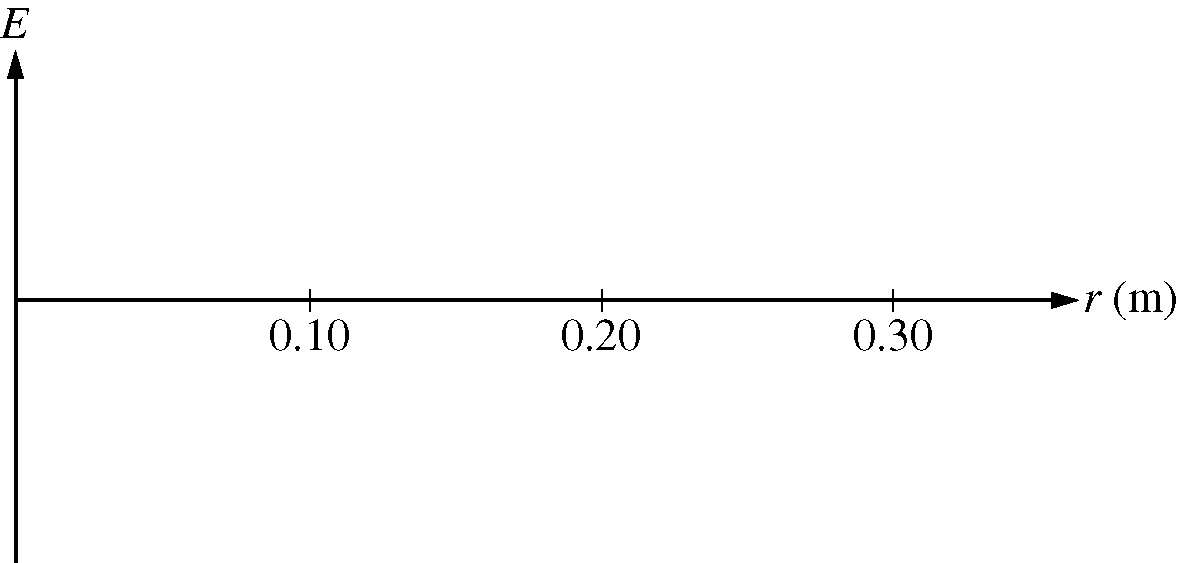
\includegraphics[scale=0.3]{images/img-015-027.png}
\end{figure}

%-------------------------------------------------------------------------------
% 请勿删除本注释
% Part (f)
%
% 指引:
% 如在小问之前有通用问题描述,请放置于此
%-------------------------------------------------------------------------------

\part
On the axes below, sketch the electric potential $V$ as a function of $r$. % 请删除并替换本行,与上一行 \part 之间不要留空行

\begin{figure}[h]
\centering
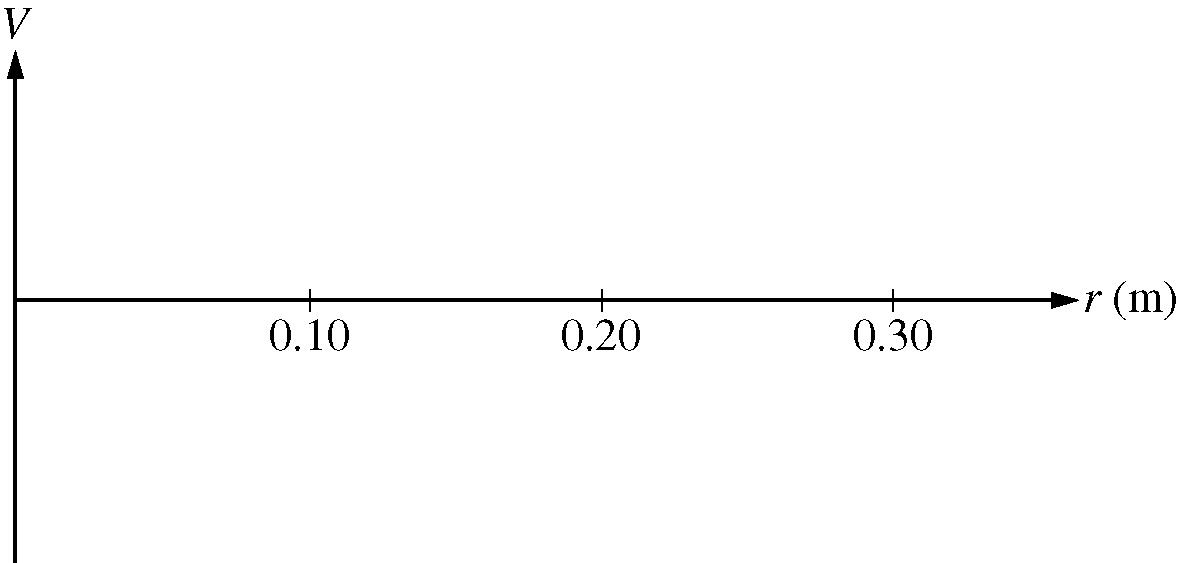
\includegraphics[scale=0.3]{images/img-015-028.png}
\end{figure}

\end{parts}
 